\begin{solution}


	\tcbsubtitle{Task A}

	\textbf{To prove: }

	\emph{Let $X$ be a continuous real-valued random variable with CDF  : $\mathbb{R} \rightarrow [0, 1]$. Assume that
		$F_X$ is invertible. Then the random variable $Y := F_X (X) \in [0, 1]$ is uniformly distributed in $[0, 1]$}

	\textbf{Proof:}\\
	$F_X$ by definition can also be written as
	\begin{align}
		F_X(x) = P(X\leq x)
	\end{align}

	Define a new random variable $Y$,
	\begin{align}
		Y =F_X(X)
	\end{align}

	Y is the result of applying CDF $F_X$ to the random variable $X$. To
	prove the theorem, assume $y\in [0,1]$. So, the probablity that $Y \leq
		y$ is:
	\begin{align}
		P(Y\leq y) = P(F_X(X)\leq y)
	\end{align}

	It is assumed that $F_X(x)$ is invertible, so,
	\begin{align}
		P(Y\leq y) = P(X\leq F_X^{-1}(y))
	\end{align}

	which is basically, probablity that $X$ is less that or equal to $F_X^{-1}(y)$. This can be written in the CDF form, which is $F_X(F_X^{-1}(y))$. So,
	\begin{align}
		P(Y\leq y) = P(X\leq F_X^{-1}(y)) = F_X(F_X^{-1}(y)) = y
	\end{align}

	So,
	\begin{align}
		P(Y\leq y) = y
	\end{align}

	where $y\in [0,1]$, which is the CDF of uniform distributon in $[0,1]$.
	So, Y is a uniform distributon in $[0,1]$ regardless of $X$.



	\tcbsubtitle{Task B}

	According to the theorem proved above, CDF of any random variable $X$
	mapped with itself gives a uniform random variable $Y$ in $[0,1]$. So,
	let $Y\sim \text{Uniform}(0,1)$. Then for any random variable $X$,
	\begin{align}
		F_X(X) & = Y           \\
		X      & = F_X^{-1}(Y)
	\end{align}

	\textbf{Algorithm $\mathcal{A}$:}
	\begin{enumerate}
		\item Input: A sample $y$ from the uniform distributon on $[0,1]$.
		\item Transformation:
		      \begin{itemize}
			      \item Apply the inverse CDF to $y$ to compute a sample $u$.
			      \item Define $\mathcal{A}(u) = u = F_X^{-1}(y)$
		      \end{itemize}
		\item Output: The random variable $U = F_X^{-1}(Y)$
	\end{enumerate}

	This gives us the correct required random variables as, CDF of U is $F_U(u)$,
	\begin{align}
		P(U\leq u ) & = P(F_X(Y) \leq u)            \\
		F_U(u)      & =  P(F_X(F_X^{-1}(X) \leq u)) \\
		F_U(u)      & =  P(X \leq u)                \\
		F_U(u)      & =  F_X(u)                     \\
	\end{align}

	$U$ and $X$ have the same CDF, which was initially required.

	\textbf{Proof:}\\
	$F_X$ by definition can also be written as
	\begin{align}
		F_X(x) = P(X\leq x)
	\end{align}

	Define a new random variable $Y$,
	\begin{align}
		Y =F_X(X)
	\end{align}

	Y is the result of applying CDF $F_X$ to the random variable $X$.
	To prove the theorem, assume $y\in [0,1]$. So, the probability that $Y \leq y$ is:
	\begin{align}
		P(Y\leq y) = P(F_X(X)\leq y)
	\end{align}

	It is assumed that $F_X(x)$ is invertible, so,
	\begin{align}
		P(Y\leq y) = P(X\leq F_X^{-1}(y))
	\end{align}

	which is basically, probability that $X$ is less that or equal to $F_X^{-1}(y)$. This can be written in the CDF form, which is $F_X(F_X^{-1}(y))$. So,
	\begin{align}
		P(Y\leq y) = P(X\leq F_X^{-1}(y)) = F_X(F_X^{-1}(y)) = y
	\end{align}

	So,
	\begin{align}
		P(Y\leq y) = y
	\end{align}

	where $y\in [0,1]$, which is the CDF of uniform distributon in $[0,1]$.
	So, Y is a uniform distributon in $[0,1]$ regardless of $X$.



	\tcbsubtitle{Task C}
	The code can be found in \texttt{2c.py}. In this script, we generate random samples from a Gaussian distribution using the inverse transform sampling method. The function \texttt{sample(loc, scale)} begins by creating a sample, \texttt{x}, which consists of uniformly distributed random variables between 0 and 1, with a sample size of \texttt{N} (where \texttt{N} = $10^5$ or 100,000).

	These uniform samples, \texttt{x}, are then transformed into samples from a Gaussian (normal) distribution by passing them through the inverse cumulative distribution function (CDF) of the normal distribution, implemented via \texttt{norm.ppf}. The arguments \texttt{loc} and \texttt{scale} represent the mean and standard deviation of the Gaussian distribution, respectively. This transformation effectively maps the uniform samples to samples drawn from the specified Gaussian distribution, as demonstrated theoretically in previous sections.

	We then define the list \texttt{params}, which contains tuples of means and variances for the Gaussian distributions we wish to sample from and plot. For each set of parameters, the \texttt{sample()} function is called, and the resulting samples are stored in the \texttt{samples} list.

	Finally, we loop over the pairs of parameters (\texttt{params}) and their corresponding samples (\texttt{samples}) to create a histogram for each distribution. The histograms are plotted with 500 bins, and the density is normalized. A legend is included to indicate the mean (\texttt{$\mu$}) and standard deviation (\texttt{$\sigma$}) for each distribution.

	Below is the resulting histogram:
	\begin{figure}[H]
		\centering
		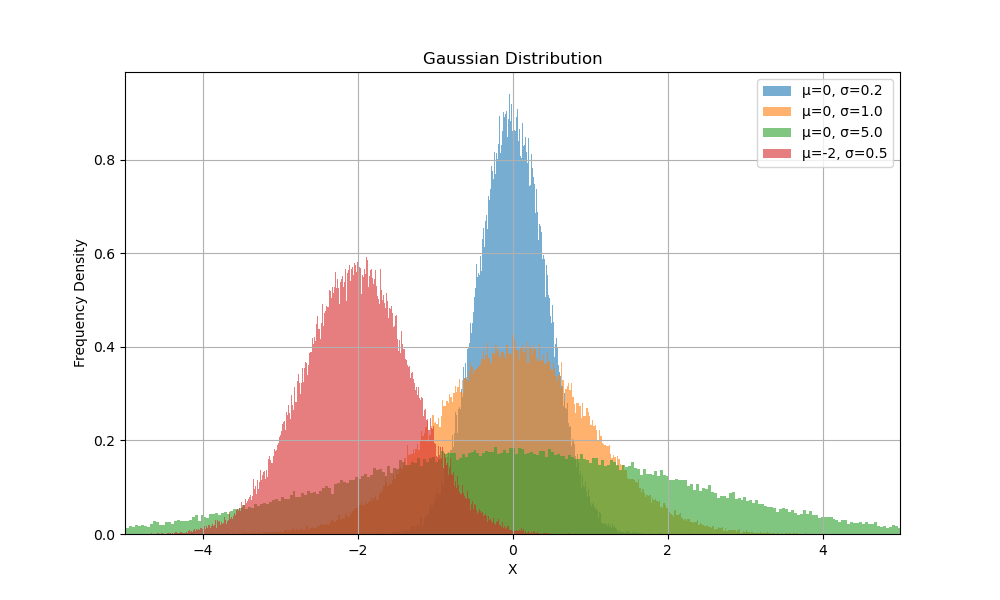
\includegraphics[width=0.8\textwidth]{../images/2c.png}
		\caption{Histograms of Gaussian distributions for different means and variances}
		\label{fig:gaussian_hist}
	\end{figure}
	
	\tcbsubtitle{Task D}
	The code for simulating the Galton board is found in \texttt{2d.py}. We implemented a function called \texttt{galton\_board}, which takes two parameters: \texttt{h}, representing the depth of the Galton board (number of pegs the ball hits), and \texttt{N}, the number of balls dropped.

Inside the function, the variable steps is a matrix with \texttt{N} rows and \texttt{h} columns. Each row corresponds to a ball, and each column represents a decision the ball makes at a peg. At each step, the ball either moves left, represented by $-1$, or right, represented by $1$. The final position of each ball is determined by summing all its steps, which is stored in the 1-D array positions. This array records the final pocket into which each ball falls.

	For the simulation, $1000$ balls are dropped for different values of \texttt{h} (the depth of the board). The resulting distributions for each value of h are visualized as histograms, with the x-axis representing the final positions (pockets) and the y-axis showing the probability of balls falling into each pocket. The results for different values of h are shown below.
	\begin{figure}[H]
		\centering
		\begin{minipage}{0.5\textwidth}
			\centering
			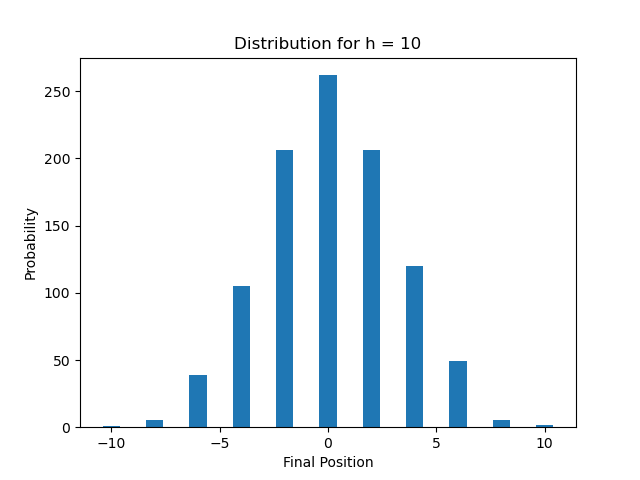
\includegraphics[width=\linewidth]{../images/2d1.png}
			\caption{Height = 10}
		\end{minipage}\hfill
		\begin{minipage}{0.5\textwidth}
			\centering
			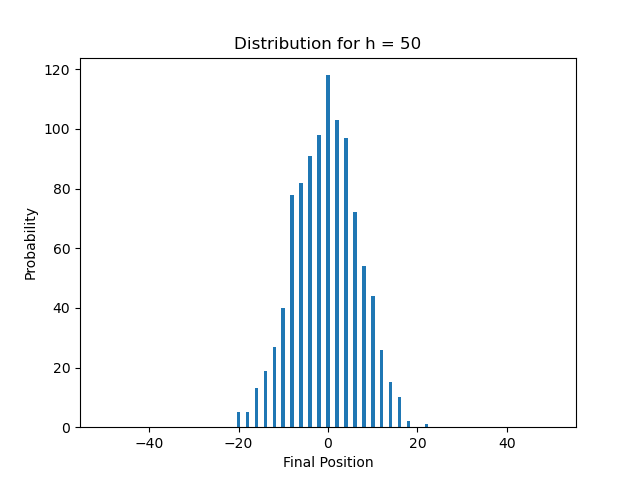
\includegraphics[width=\linewidth]{../images/2d2.png}
			\caption{Height = 50}
		\end{minipage}\hfill		
	\end{figure}
	\begin{figure}[H]
		\centering
		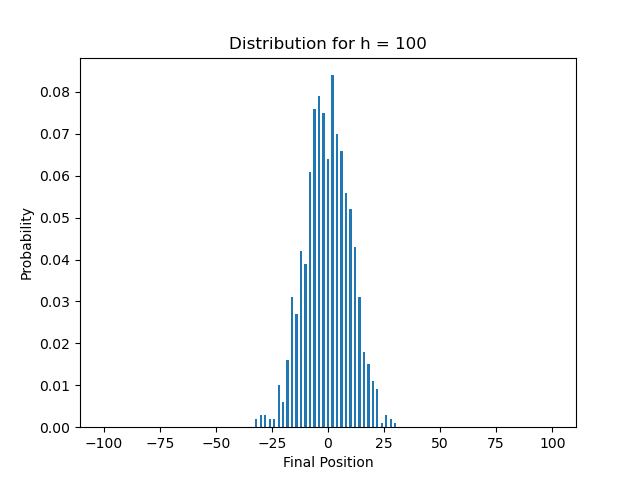
\includegraphics[width=0.8\textwidth]{../images/2d3.png}
		\caption{Height = 100}
		
	\end{figure}

	The shape of the tops of the histogram closely resembles a Gaussian distribution. As the height (\texttt{h}) of the Galton board increases, the distribution becomes smoother and more bell-shaped, indicating that most balls tend to fall around the center pockets.

	\tcbsubtitle{Task E(B)}
	We have a random variable $X$ which can take values from
	$\{-h,-h+2,\ldots,h-2,h\}$. Each ball makes $h$ random binary
	decisions(left or right) as it descends. If we let $Y$ be the number of
	times the ball moves right, the final position of the ball will be
	given by,
	\begin{align}
		X = -h+2Y
	\end{align}

	where $Y$ is a \textbf{binomial variable} because in simple terms it is the summation of $h$ bernoulli decisions each with probability $\frac{1}{2}$.
	\begin{align}
		Y \sim \Bin(h,\frac{1}{2})
	\end{align}

	For a particular pocket $X = 2i$, the corresponding value of Y is:
	\begin{align}
		Y = \frac{h+2i}{2}
	\end{align}

	Thus, the probability that the ball lands in the pocket $X=2i$ is the
	probability that $Y = \frac{h+2i}{2}$. Using Binmial distribution, this
	is:
	\begin{align}
		P_h[X=2i]=P_h\left[Y=\frac{h+2i}{2}\right]=\binom{h}{\frac{h+2i}{2}}\left(\frac{1}{2}\right)^h
	\end{align}

	This is the \textbf{closed form expression for $P_h[X=2i]$}

	Now, we need to show $P_h[X=2i]$ approximates to normal distribution for very large $h$.\\
	Using \textbf{stiriling's approximation} for large $n$, which states that:
	\begin{align}
		n!\approx \sqrt[]{2\pi n}\left(\frac{n}{2}\right)^n
	\end{align}
	We can convert the factorials in the binomial coefficient:
	\begin{align}
		\binom{h}{r} \approx \frac{h!}{r!(h-r)!}
	\end{align}
	Using stirlings approximation, we have,
	\begin{align}
		\binom{h}{y} = \frac{\sqrt[]{2\pi h}\left(\frac{h}{e}\right)^h}{\sqrt[]{2\pi y}\left(\frac{y}{e}\right)^y\cdot \sqrt[]{2\pi(h-y)}\left(\frac{h-y}{e}\right)^{h-y}}
	\end{align}
	where $y = \frac{h+2i}{2}$
	For large $h$, we can simplify this assuming small $i$ (relative to $h$). In particular, $\frac{h+2i}{2}$ can be written as $\frac{h}{2}$, leading to:
	\begin{align}
		\binom{h}{\frac{h+2i}{2}} \approx \frac{2^h}{\sqrt[]{\pi h}}e^{-\frac{2i^2}{h}}
	\end{align}
	Substituting it back in $P_h$ gives:
	\begin{align}
		P_h[X=2i]\approx \frac{2^h}{\sqrt[]{\pi h}}e^{-\frac{2i^2}{h}}\left(\frac{1}{2}\right)^h
	\end{align}
	Simplifying the powers of 2 gives:
	\begin{align}
		P_h[X=2i]\approx \frac{1}{\sqrt[]{\pi h}}e^{-\frac{2i^2}{h}}
	\end{align}
	which is basically normal distribution with $\mu = 0$ and $\sigma^2=h/2$
\end{solution}
